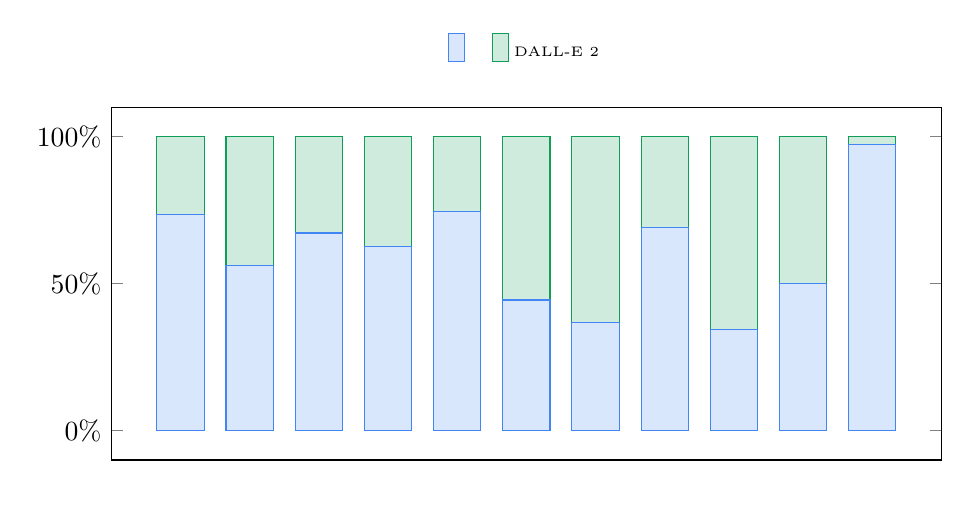
\begin{tikzpicture}

\definecolor{google_blue}{RGB}{66,133,244}
\definecolor{google_red}{RGB}{219,68,55}
\definecolor{google_yellow}{RGB}{194,144,0}
\definecolor{google_green}{RGB}{15,157,88}

\begin{axis}[
name=fidelity,
width=\textwidth,
height=0.5\textwidth,
ybar stacked,
ymin=-0.1,
ymax=1.1,
xtick=data,
xtick style={draw=none},
symbolic x coords={Colors,Conflicting,Counting,DALL-E \cite{ramesh-dalle},Descriptions,Marcus et al. \cite{marcus-arxiv-2022},Misspellings,Positional,Rare Words,Reddit,Text},
xticklabels={},
x tick label style={rotate=30},
ytick={0,0.5,1},
yticklabels={0\%, 50\%, 100\%},
legend style={font=\tiny},
legend cell align=left,
legend image code/.code={
    \draw [#1] (0cm, -0.1cm) rectangle (0.2cm, 0.25cm);
},
legend style={
draw=none,
at={(0.5, 1.1)},anchor=south,
legend columns=3,
/tikz/every even column/.append style={column sep=0.2cm}
},
bar width=0.6cm,
]

\addplot+[
    fill=google_blue,
    fill opacity=0.2,
    draw=google_blue
] coordinates {
(Colors, 0.736)
(Conflicting, 0.562)
(Counting, 0.672)
(DALL-E \cite{ramesh-dalle}, 0.627)
(Descriptions, 0.746)
(Marcus et al. \cite{marcus-arxiv-2022}, 0.444)
(Misspellings, 0.369)
(Positional, 0.691)
(Rare Words, 0.344)
(Reddit, 0.499)
(Text, 0.972)
};

\addplot+[
fill=google_green,
fill opacity=0.2,
draw=google_green
] coordinates {
(Colors, 0.264)
(Conflicting, 0.438)
(Counting, 0.328)
(DALL-E \cite{ramesh-dalle}, 0.372)
(Descriptions, 0.254)
(Marcus et al. \cite{marcus-arxiv-2022}, 0.556)
(Misspellings, 0.631)
(Positional, 0.309)
(Rare Words, 0.655)
(Reddit, 0.501)
(Text, 0.028)
};

\legend{\name, DALL-E 2}
\end{axis}

\end{tikzpicture}